\documentclass[compress]{beamer}

\usepackage[utf8]{vntex}
\usepackage{longtable}
\usepackage{amsmath}
\usepackage{amsmath}
\usepackage{amsfonts}
\usepackage{cases}
\usepackage{amssymb}
\usepackage[utf8]{inputenc}
\usepackage[absolute,overlay]{textpos}
\usepackage{listings}

\lstset{
	language = Java,
	frame = single,
	tabsize = 3
}

\usetheme{Warsaw}
%\usetheme{Antibes}
%\usecolortheme{spruce}
%\setbeamercolor{structure}{fg=cyan!90!blue}
%\newtheorem{theorem}{Định lý}[]

\expandafter\def\expandafter\insertshorttitle\expandafter{%
    \insertshorttitle\hfill%
    \insertframenumber\,/\,\inserttotalframenumber}
      
\AtBeginSection[] % Do nothing for \section*
{
\begin{frame}
\tableofcontents[currentsection]
\end{frame}
}
\AtBeginSubsection[] % Do nothing for \section*
{
\begin{frame}
\tableofcontents[currentsection, currentsubsection]
\end{frame}
}

\title[Evolutionary Multitasking]{Evolutionary Multitasking} 

\author[Nguyễn Tuấn Đạt, Phan Anh Tú (SoICT-HUST)]{
Sinh viên thực hiện\\
Nguyễn Tuấn Đạt - 20130856 \\
Phan Anh Tú - 20134501 \\[0.5cm]
Giảng viên \\
PGS.TS Huỳnh Thị Thanh Bình
}

\begin{document}

\begin{frame}[plain]
\titlepage
\end{frame}

\begin{frame}[plain]{Nội dung trình bày}
\tableofcontents
\end{frame}

\section{Giới thiệu bài toán}

\begin{frame}{Giới thiệu}
\begin{itemize}
\item Giải thuật tiến hóa: là một giải thuật tối ưu hóa metaheuristics ý tưởng dựa trên thuyết tiến hóa của Đác-uyn.
\pause
\item Cách thức hoạt động của thuật toán:
\pause
\begin{itemize}
\item Từ một quần thể ban đầu các cá thể được cho đi lai ghép và đột biến để tạo ra các cá thể con.
\item Quần thể sẽ chọn lọc các cá thể tốt nhất để đi đến thế hệ sau.
\item Thuật toán sẽ lặp đi lặp lại qua một số lượng thế hệ nhất định để chọn được cá thể tốt nhất.
\end{itemize}
\end{itemize}
\framesubtitle{Giới thiệu chung}
\end{frame}
\begin{frame}{Tiến hóa đa nhiệm}
\framesubtitle{Evolutionary Multitasking}
\begin{block}{Tiến hóa đa nhiệm}
Nhiều công việc cùng được tối ưu trong một quá trình tiến hóa.
\end{block}
\pause
\begin{block}{Lợi ích}
\begin{itemize}
\item Các quá trình tối ưu ứng với các công việc khác nhau trong tiến hóa đa nhiệm vụ có thể phần nào đó bổ xung, hỗ cho nhau.
\item Giúp tăng gia tốc tốc tối ưu trong các vấn đề phức tạp
\begin{itemize}
\item Chuyển dịch hiểu biết
\item Tăng năng xuất ( nhiều quá trình tối ưu thành 1 quá trình tối ưu )
\end{itemize}
\end{itemize}
\end{block}

\end{frame}
\begin{frame}{Tiến hóa đa nhiệm}
\framesubtitle{Evolutionary Multitasking}
\begin{exampleblock}{Vấn đề }
\begin{itemize}
\pause
\item Cân nhắc vị trí các công việc cần giải quyết như thế nào trong chỉ một quá trình tiến hóa ?
\pause
\item Hàm thích nghi phải làm hàm như thế nào? 
\pause
\item Làm sao để các công việc đều được tối ưu?
\end{itemize}
\end{exampleblock}
\end{frame}
\begin{frame}{MFO}
\framesubtitle{Multifactorial Optimization}
\begin{block}{MFO}
\begin{itemize}
\item Một sơ đồ tiến hóa hỗn hợp (đa nhiệm vụ)khi phát triển quần thể  thực chất ẩn chứa một quá trình song song để tối ưu nhiều các công việc khác nhau trên cùng một quần thể.
\pause
\item MFO là một sơ đồ tiến hóa đa nhiệm mà ở đó mỗi công việc tối ưu được nhìn như là một nhân tố ảnh hưởng đến quá trình tiến hóa.
\end{itemize}
\end{block}
\end{frame}
\begin{frame}{MFO}
\framesubtitle{Multifactorial Optimization}
\begin{itemize}
\item Xét k công việc cần tối ưu \textit{K- task}
\item \textit{$i^{th}$ task} ta có hàm mục tiêu $f_i: X_i \longrightarrow R$
\item Mục tiêu của \textit{MFO}: 
$$\{x_1, x_2, \ldots x_K\}= argmin\{f_1(x), f_2(x), \ldots f_K(x)\}$$
\end{itemize}
\end{frame}

\section{Thuật toán}
\begin{frame}{Một vài định nghĩa}
\onslide<1->{
\begin{block}{Factorial rank}
Factorial rank $r_{ij}$ là rank của cá thể $p_i$ trên task $T_j$
\end{block}}
\onslide<2->{\begin{block}{Scalar fitness} 
${\varphi}_i$ của cá thể $p_i$ phụ thuộc vào rank tốt nhất của nó trên tất cả các task. (VD: ${\varphi}_i = 1/min\{r_{i1}, r_{i2}, ..., r_{iK}\}$)
\end{block}}
\onslide<3->{\begin{block}{Skill factor}
Skill factor ${\tau}_i$ của cá thể $p_i$ là chỉ số của một task có rank cao nhất trong $K$ task của $p_i$ (${\tau}_i = argmin_j\{r_{ij}\}$)
\end{block}}
\end{frame} 

\begin{frame}{Biểu một cá thể}
\begin{itemize}
\onslide<1->\item Một lời giải của task $i^{th}$ biểu diễn bởi vector có chiều $D_i$
\onslide<2->\item Biểu diễn cá thể bằng một vector có số chiều = $max\{D_i\}$ và giá trị nằm trong khoảng $[0,1]$
\onslide<3->\item Biểu diễn 2 task: 
\begin{itemize}
\onslide<3->\item 12-D Knapsack 
\onslide<3->\item 6-D TSP 
\onslide<4->{\begin{longtable}{|c|c|c|c|c|c|c|c|c|c|c|c|}
\hline
0.8 & 0.9 & 0.1 & 0.9 & 0.6 & 0.0 & 0.2 & 0.5 & 0.9 & 0.4 & 0.1 & 0.9\\
\hline
\end{longtable}}
\end{itemize}
\onslide<5->\item Decode
\begin{itemize}
\onslide<6->\item Knapsack
\onslide<7->{\begin{longtable}{|c|c|c|c|c|c|c|c|c|c|c|c|}
\hline
1 & 1 & 0 & 1 & 1 & 0 & 0 & 0 & 1 & 0 & 0 & 0\\
\hline
\end{longtable}}
\onslide<6->\item TSP
\onslide<8->{\begin{longtable}{|c|c|c|c|c|c|}
\hline
6 & 3 & 5 & 1 & 2 & 4\\
\hline
\end{longtable}}
\end{itemize}
\end{itemize}
\end{frame}

\begin{frame}{Cải tiến Decode}
\begin{itemize}
\onslide<1->\item Nhận xét: Decode bài toán có kích thước nhỏ hơn, lấy n phần tử đầu của cá thể -> Không lấy được hết đặc trưng của cá thể
\onslide<2->\item Cải tiến: Sử dụng window trượt qua các phần tử trong cá thể
\onslide<3->{\begin{longtable}{|c|c|c|c|c|c|}
\hline
$x_1$ & $x_2$ & $x_3$ & ... & $x_4$ & $x_5$ \\
\hline
\end{longtable}}
\onslide<4->{\begin{longtable}{|c|c|c|}
\hline
$w_1$ & $w_2$ & $w_3$\\
\hline
\end{longtable}}
\onslide<4->{\begin{longtable}{|c|c|c|}
\hline
$x_1*w_1+x_2*w_2+x_3*w_3$ & ... & $x_i*w_1+x_{i+1}*w_2+x_{i+2}*w_3$\\
\hline
\end{longtable}}

\onslide<5->{$$D' = (D-F+P)/S + 1$$}
\begin{itemize}
\onslide<6->\item $D'$ : số chiều sau khi decode
\onslide<7->\item $D$ : số chiều của cá thể, $F$ : độ rộng của window
\onslide<8->\item $P$ : số lượng số 0 được thêm vào cá thể 
\onslide<9->\item $S$ : số ô nhảy qua  
\end{itemize}
\end{itemize}
\end{frame}

\begin{frame}{Thuật toán}
\begin{figure}
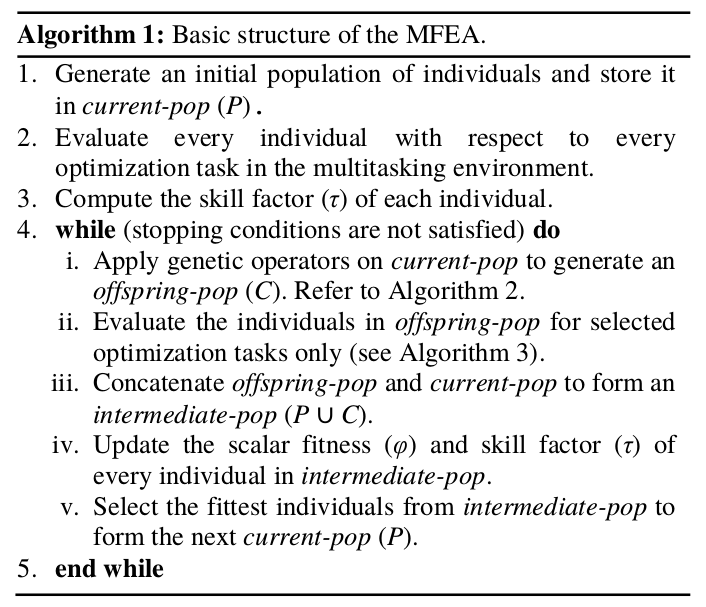
\includegraphics[scale=0.45]{al1.png}
\end{figure}
\end{frame}

\begin{frame}{Thuật toán}
\begin{figure}
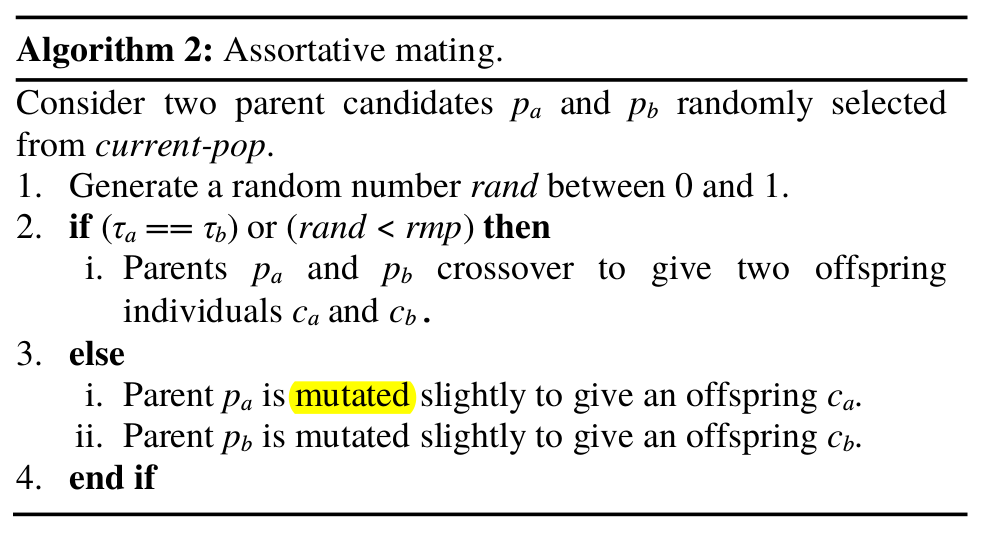
\includegraphics[scale=0.45]{al2.png}
\end{figure}
\end{frame}

\begin{frame}{Thuật toán}
\begin{figure}
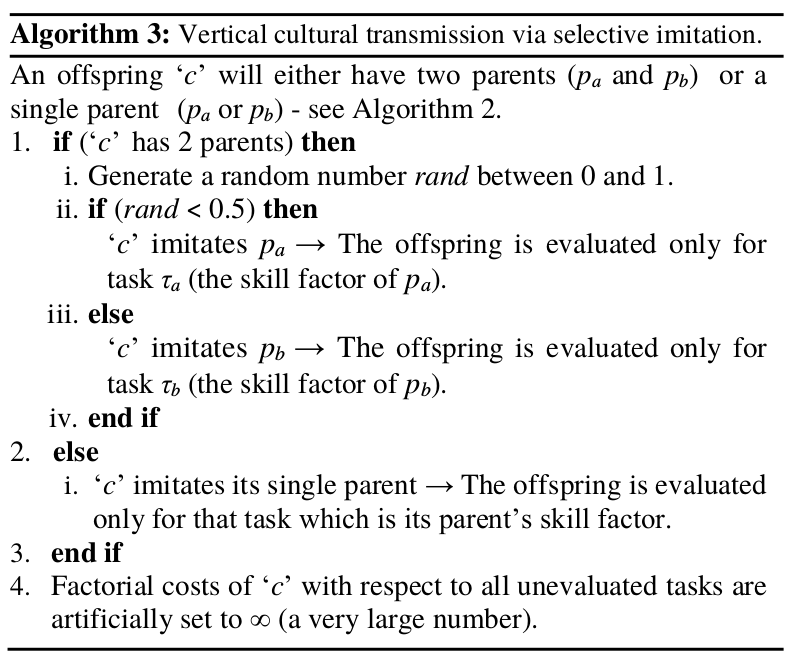
\includegraphics[scale=0.42]{al3.png}
\end{figure}
\end{frame}

\begin{frame}[plain]{Thank you for attention! Any Question?}
Hope you enjoy!
\end{frame}

\end{document}
